\subsection{Introduction}
%
Google Cloud Platform is one of the most used public cloud platforms and is still continuing to grow. It offers a cloud services that run on same infrastructure that Google hosts their product such as Google search, Gmail and Youtube. After Launching of Google App Engine, we have seen other services introduced and the list is continuing to rise.
%
% \subsection{CI-CD Process}
%
% How to setup CI-CD on the tool?


\subsection{Setting up a CI/CD pipeline for data-processing workflow}
%
Setting up a continuous integration/continuous deployment is done by implementing CI/CD methods with manage products on Google cloud. It ensures high quality,maintainability and adaptability of data process and workflows.The methods are as follows:
\begin{itemize}
    \item Version Control of source code.
    \item Automatic building,testing and deployment of apps.
    \item Environment isolation and separation from production.
    \item Replicable procedures for environment setup.
\end{itemize}
%
\subsection{Deployment Architecture}
%
\begin{itemize}
    \item  \textbf{Cloud Build} to create a CI/CD pipeline for building, deploying, and testing a data-processing workflow,as well as the data processing itself. It is a managed service that uses Google Cloud to run the build. A build is a collection of build steps, each of which is run in its own Docker container.
    \item \textbf{Cloud Composer} is used to define and run workflow steps such as data processing, testing, and verification. It is a managed Apache Airflow service that allows you to create, schedule, monitor, and manage complex workflows.
    \item \textbf{Dataflow} is the serverless execution service from GCP for data-processing pipelines written using Apache Beam. Apache Beam is an open-source, unified model for defining both batch and streaming data-parallel processing pipelines.
\end{itemize}

\subsubsection{The CI/CD pipeline}
%
At a high level, the CI/CD pipeline consists of following steps:
\begin{itemize}
    \item Cloud Build packages the sample application into a JAR file using the Maven Builder. The Maven Builder is a container with Maven installed in it.Maven runs the task When a build step is configured to use the Maven Builder
    \item Cloud Build uploads the JAR file to cloud storage
    \item Cloud Build runs unit tests on data-processing workflow code and deploys the workflow code to the Cloud Composer.
    \item Cloud Composer picks up the JAR file and runs the data-processing job on Data-flow. 
\end{itemize}

% 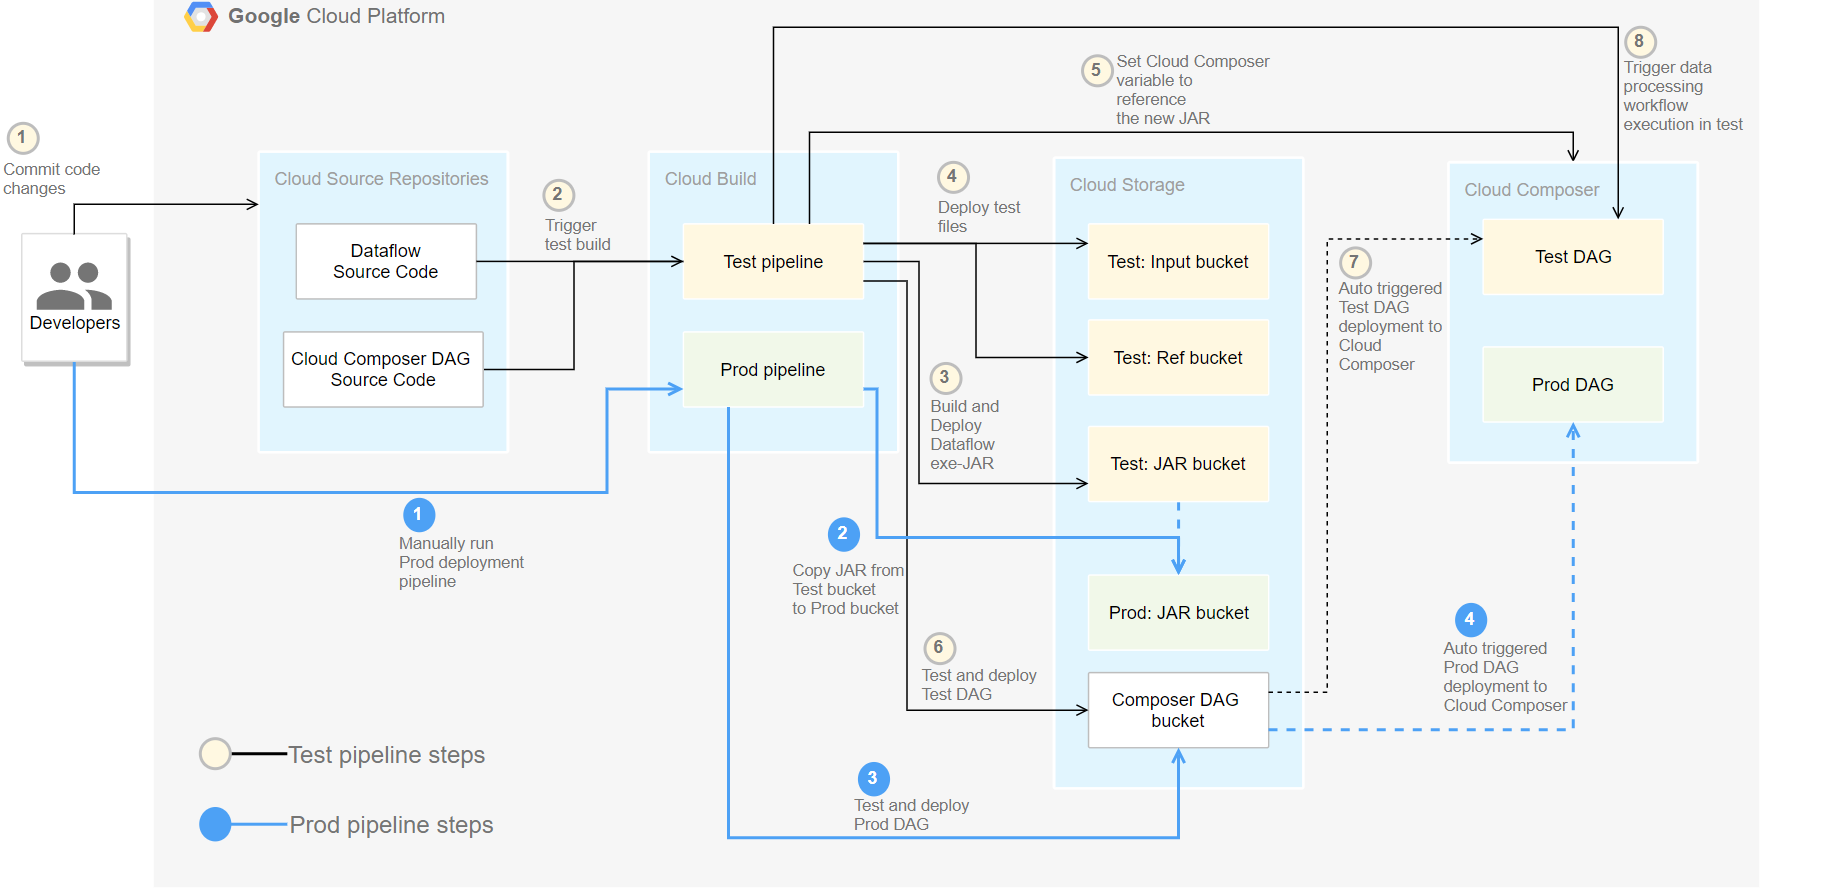
\includegraphics[scale=0.55]{images/cicd-pipeline-for-data-processing-1-diagram-pipeline.png}

\begin{figure}[h]
    \centering
    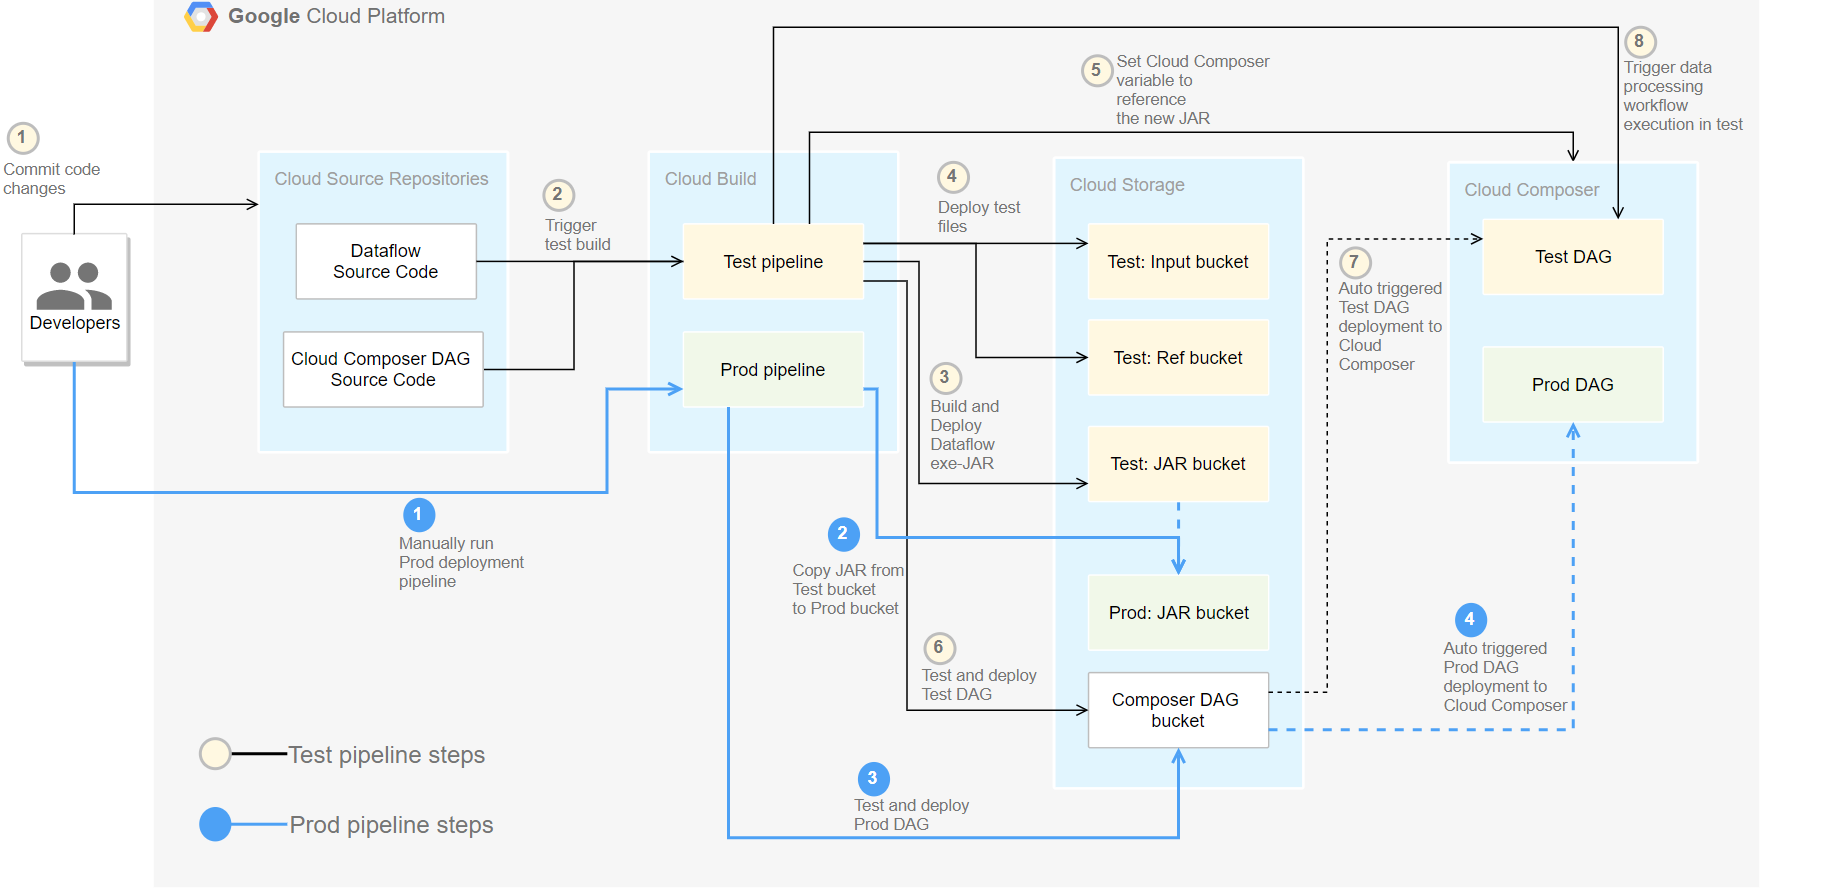
\includegraphics[scale=0.53]{images/cicd-pipeline-for-data-processing-1-diagram-pipeline.png}
    \caption{Workflow of CI/CD pipeline in GCP.} 
    \label{fig:gcp_cicd}
\end{figure}



\newline\newline\newline
We can see in the figure~\ref{fig:gcp_cicd},  the deployments to the test and production environments are separated into two different cloud Build pipelines- a test and a production pipeline.\footnote{https://cloud.google.com/architecture/cicd-pipeline-for-data-processing\#the\_cicd\_pipeline} 
\newline\newline     In the preceding diagram, the test pipeline consists of the following steps: 
\begin{enumerate}
    \item A developer commits code changes to the Cloud Source Repositories. 
    \item Code changes trigger a test build in cloud build.
    \item Cloud Build builds the self-executing JAR file and deploys it to the test JAR bucket on cloud storage. 
    \item Cloud Build deploys the test files to the test-file buckets on cloud storage.
    \item Cloud Build sets the variable in Cloud Composer to reference the newly deployed JAR file. 
    \item Cloud Build tests the the data processing workflow Directed Acyclic Graph(DAG) and deploys it to the Cloud Composer bucket on Cloud Storage.
    \item The workflow DAG file is deployed to Cloud Composer 
    \item Cloud Build triggers the newly deployed data-processing workflow to run. 
\end{enumerate}
\newline
In the preceding diagram, the production pipeline consists of the following steps: 
\begin{enumerate}
    \item A Developer manually runs the production deployment pipeline in Cloud Build.
    \item Cloud Build copies the latest self-executing JAR file from the test JAR bucket to the production JAR bucket on cloud storage. 
    \item Cloud Build tests the production data processing workflow DAG and deploys it to the Cloud Composer bucket on Cloud Storage. 
    \item The production workflow DAG file is deployed to Cloud Composer.
\end{enumerate}


%
%
\subsection{Pricing}
%
Google Cloud Platform has no up-front costs, pay-as-you-go services, and no fees for termination. In addition, GCP stands out for for its discounts. 
%
\subsection{Advantages}
%
GCP probably benefits from the simple fact that it is owned by google. Apart from that, there are some benefits of using GCP. 
\begin{itemize}
    \item Google Cloud Platform(GCP) is designed for cloud-native businesses
    \item Commitment to open source and portability
    \item Deep discounts and flexible contracts
 \item DevOps expertise

\end{itemize}
%
\subsection{Disadvantages}
%
GCP has some disadvantages like other platform.

\begin{itemize}
    \item GCP is still continuing to grow.
    \item It has less feature and service than AWS and Microsoft Azure. 
\end{itemize}
%